% Template for Cogsci submission with R Markdown

% Stuff changed from original Markdown PLOS Template
\documentclass[10pt, letterpaper]{article}

\usepackage{cogsci}


\title{Not so opaque after all: Conventions formed in reference games
are mostly understandable to outsiders}

\usepackage{booktabs}

\author{{\large \bf Veronica Boyce (vboyce@stanford.edu)} \\ Department of Psychology \\ Stanford University \And {\large \bf Ben Prystawski (benpry@stanford.edu)} \\Department of Psychology \\ Stanford University \AND {\large \bf Alvin Wei Ming Tan (tanawm@stanford.edu)} \\ Department of Psychology \\ Stanford University \And {\large \bf Michael C. Frank (mcfrank@stanford.edu)} \\ Department of Psychology \\ Stanford University}


\begin{document}

\maketitle

\begin{abstract}
In-groups can create conventionalized language, but this jargon may in
fact be understandable to those outside the group. The formation of
temporary linguistic conventions between individuals is often studied in
iterated reference games, where over repeated reference to the same
targets, a describer--matcher pair establishes partner-specific
shorthand names for targets. One open question is how understandable
these referring expressions are to others who were not part of the
convention formation process. We take an outside angle on understanding
convention formation, using experiments with naïve matchers and
computational models to assess the opacity of descriptions from iterated
reference games. Both human matchers and the computational model are
well above chance accuracy, with variation in performance primarily
driven by the target image rather than where or when the description
came from. This additional perspective can inform work on how
conventions are formed and how efficient such conventions actually are.

\textbf{Keywords:}
reference games; convention formation; computational modeling; opacity
\end{abstract}

\section{Introduction}\label{introduction}

Groups of people often have terms that are used within a group, such as
regional dialects, field-specific jargon, or terms of art related to
specific theoretic orientations. Those who are not part of the group may
use different terms for the same targets, but may nonetheless be able to
understand or guess at the meanings of in-group terms. While these terms
can represent stable conventions shared by sizable communities,
temporary naming conventions can also develop rapidly among small groups
of people when there is a need to refer to something without a canonical
name that distinguishes it in context.

This formation of temporary linguistic conventions between individuals
is often studied in iterated reference games. In these games, a
describer tells their partner how to sort or match a series of abstract
images (e.g., Clark \& Wilkes-Gibbs, 1986; Hawkins et al., 2020). Over
repeated rounds of referring to the same targets, pairs usually develop
conventionalized nicknames for the target images. These nicknames are
often partner-specific, in that different pairs develop different
nicknames for the same targets. When describing the shapes for people
who were not part of the group, people return to more elaborated
descriptions, indicating an expectation that others may be unable to
understand the convention, and need a longer or different referential
description (Hawkins et al., 2021; Wilkes-Gibbs \& Clark, 1992; Yoon \&
Brown-Schmidt, 2018). Participants treat later-stage conventions as more
opaque to outsiders than earlier-stage descriptions, and the
differentiation of labels across groups over time is a signal of
arbitrariness in the conventions (Boyce et al., 2024; Hawkins et al.,
2020).

How arbitrary and opaque are these conventions, really? One way to
conceptualize the opacity of a referring expression is by considering
the semantic distance between the signifier and the referent. Under the
assumption of a modality-independent global semantics (i.e., not
conditioned by partner-specific meaning), expressions that are
transparent have signifiers and referents that are semantically close,
such that any member of the sociolinguistic community sharing the global
semantics should be able to identify the appropriate referent given the
signifier. In contrast, expressions that are opaque have signifiers and
referents that are semantically distant, such that the relations between
them are more arbitrary and inaccessible to the general community
without the formation of additional conventions (which may be partner-
or group-specific).

Assessing opacity thus requires us to have a measure of
modality-independent global semantics. Such semantics are difficult to
directly obtain for humans, since we rarely have explicit semantic
formulations of stimuli, much less formulations that are unified across
multiple modalities. However, another approach is to look at how
understandable conventions are to others who were not part of the
interaction that originated the convention. The ability of a naïve
comprehender to understand a referring expression presented without
context provides a proxy measure, since the comprehender's judgements
are not conditioned on any context-specific conventions. Conventions
that are more arbitrary and opaque should thus be harder for naïve
matchers to understand, and we can determine how the features of the
utterances and the conditions they were produced under affect their
opacity, providing empirical tests of whether descriptions become more
opaque over the course of the reference game.

Some prior work has investigated how well naïve matchers can understand
the descriptions produced in the course of an iterated reference game,
with a focus on the role of conversational shared history. Murfitt \&
McAllister (2001) recorded descriptions from 8 participants who
described shapes either solo or in a matching game with a partner and
played the descriptions to new matchers, either in order or in reverse
order. Naïve listeners were more accurate when the heard descriptions in
order. Schober \& Clark (1989) found that matchers in an iterated
reference game achieved higher accuracies than overhearers who listened
to the entire game in order, and overhearers who listened to recordings
starting in the third round did even worse. Nonetheless, all matchers
were far above chance, and their accuracies rose over rounds. Leung et
al. (2024) had adults and children serve as naïve matchers, listening to
descriptions from the the first and last rounds of a parent--child
iterated reference game. They found no significant difference in how
comprehensible early and late descriptions were to naïve matchers, and
while naïve matchers had high accuracy, they were slightly less accurate
than in-game matchers overall.

In an iterated reference game using drawing (rather than text) as the
communication modality, Hawkins et al. (2023) compared the accuracy of
in-game matchers to naïve matchers in yoked and shuffled conditions. The
yoked matchers saw all the trials from one game in order, while the
shuffled matchers saw trials sampled from 10 games but in trial order.
In-game matchers were more accurate overall than yoked matchers who were
in turn more accurate than shuffled matchers. Over the course of trials,
both in-game and yoked matchers showed steeper improvement in accuracy
than shuffled matchers.

Across the prior literature, while naïve matchers have worse accuracy
than in-game matchers, their performance is still far above chance,
suggesting that the convention--target relationship is not purely
arbitrary. In fact, even when pairs of participants try to obfuscate
their meaning to match images with each other but not an overhearer, an
overhearing participant can still do quite well (Clark \& Schaefer,
1987). Nonetheless, receiving more context from an interaction---and in
particular, having that context be in order---is beneficial to matchers.
Except for the shuffled condition of Hawkins et al. (2023), these
studies do not address how opaque descriptions from different points in
the game are without prior context. Such an approach would be important
to have truly naïve matchers that lack even the context of trial order,
providing a clearer understanding of opacity.

Another possible measure of modality-independent global semantics is
computational in origin. Computational methods have enabled the
embedding of various stimuli (including images and text) into
high-dimensional feature spaces; these embeddings have properties which
suggest that they are reasonable approximations of humans' semantic
spaces, including similarity in representational geometries (e.g., Grand
et al., 2022; Muttenthaler \& Hebart, 2021). Indeed, embeddings from
neural network models have been used as a form of semantics in a range
of reference game scenarios (e.g., Gul \& Artzi, 2024; Ji et al., 2022;
Kang et al., 2020; Le et al., 2022; Ohmer et al., 2022). In particular,
such embeddings can be treated as context-independent semantic
representations, since they are not updated to account for convention
formation within an iterated reference game; hence, they can serve as a
computational comparison to human performance on a naïve matching task.

In the current work, we address how the process of convention formation
shapes the levels of opacity of the referring expressions created at
different time points in an iterated reference game. Using reference
expressions created in different games from Boyce et al. (2024), we use
both human experiments and models to assess when and why expressions are
opaque or understandable to outside observers.

\begin{CodeChunk}
\begin{figure}[t!]

{\centering 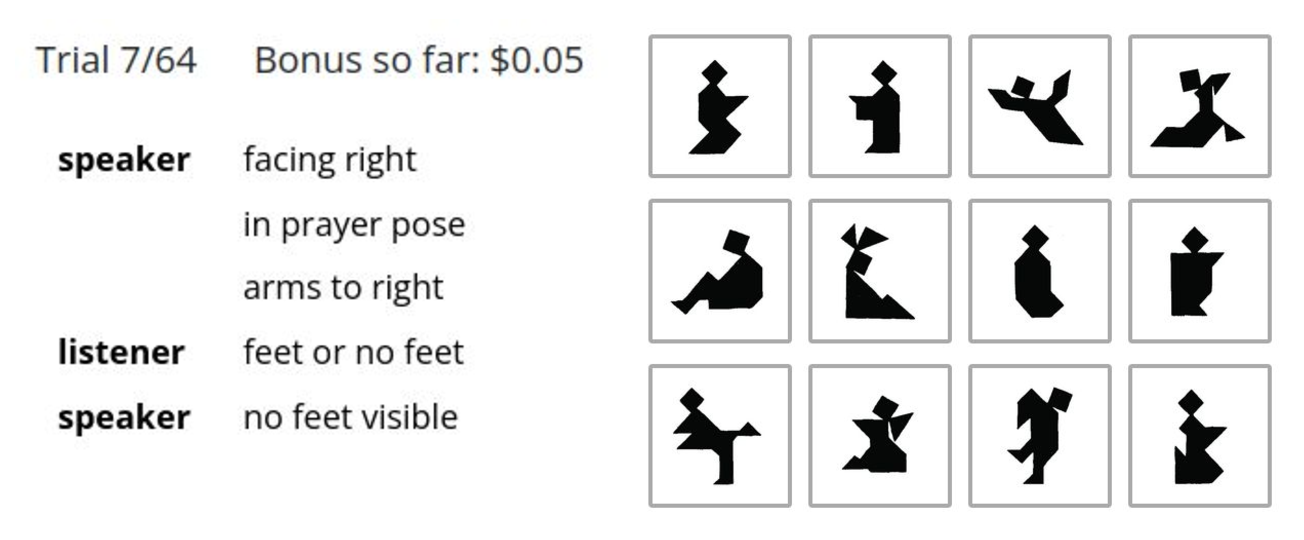
\includegraphics[width=1\linewidth]{matcher-diagram} 

}

\caption[Experimental Setup]{Experimental Setup. Naive matchers read transcripts from trials in reference games from Boyce et al. (2024) and selected which image they thought was being described. Matchers recieved bonus payments for correct selections. \label{game}}\label{fig:interface}
\end{figure}
\end{CodeChunk}

\section{Task setup}\label{task-setup}

\subsection{Materials}\label{materials}

We drew on the corpus of reference game transcripts and results from
Boyce et al. (2024). This corpus is made up of 6-round iterated
reference games using the same 12 target images. Games were played in
conditions varying in how large the describer--matcher groups were (2--6
participants) and how ``thick'' the communication channels were. For our
naïve matcher experiments, we sampled different subsets of this corpus.
In presenting the transcripts, we excluded utterances that were marked
by Boyce et al. (2024) as not containing any referential content
(i.e.~purely greetings, meta-commentary, or off-topic chitchat). Within
the samples, we also did not show transcripts that contained swear words
or crude or sexual language. We used the entire corpus for our
computational modeling component.

\subsection{Experimental procedure}\label{experimental-procedure}

We recruited English-speaking participants from Prolific. Participants
were directed to the experiment, where the task was explained to them.
On each trial, participants saw the full transcript from that trial,
containing all the chat messages marked by whether they were from the
speaker or a listener. Participants selected the image they thought was
the target from the tableau of 12 (Figure \ref{game}). Participants
received feedback on whether they were right or wrong on each trial.
Except when the specific viewing order was part of the experimental
manipulation, we randomized the order of trials, subject to the
constraint that the same target could not repeat on adjacent trials. The
task was implemented in jsPsych (Leeuw et al., 2023). We paid
participants \$10 an hour plus a bonus of 5 cents per correct response.
All our experimental code is at TODO LINK.

\subsection{Computational models}\label{computational-models}

We used CLIP (\texttt{clip-vit-large-patch14}) as a listener model for
our domain (Radford et al., 2021). CLIP is a natural choice for
reference games, as the model is trained to estimate the correspondence
between images and phrases in natural language. We pre-processed the
text by concatenating all the messages sent by the speaker for a given
trial, and ran CLIP for the concatenated text and all 12 tangram shapes.
We then computed probabilities for each tangram shape using CLIP's
logits. The simplest way to do this is simply taking the softmax of the
logits. However, the tangram shapes were possibly out the distribution
for the model, which led it to favor some images over others regardless
of the content of the text. To fix this, we trained readout models that
made more calibrated predictions using CLIP's logits.

\begin{table}
\caption{Cross-validated accuracies for classifiers. Standard deviations in accuracy across the 10 folds are shown in parentheses. Best performance within each model class is underlined, and best overall performance is bolded.}
\label{tab:classifier_comparison}
\centering

  \begin{tabular}{p{1em}lr}
    \toprule
    \multicolumn{2}{l}{Classifier} & Accuracy \\ 
    \midrule
        \multicolumn{2}{l}{Random baseline} & \smash{0.08} \\
    \multicolumn{2}{l}{CLIP without readout} & \smash{0.31} \\
    \multicolumn{2}{l}{Logistic regression} & \\
    & No penalty & \underline{\smash{0.50 (0.01)}} \\ 
    & \vspace{1mm}L2 penalty & 0.50  (0.01) \\ 
    \multicolumn{2}{l}{Random forest} & \\
    & 10 estimators & 0.46 (0.02) \\
    & 50 estimators  & 0.51 (0.02)\\ 
    & 100 estimators & 0.52 (0.02) \\ 
    & \vspace{1mm}500 estimators & \underline{\smash{0.52 (0.02)}} \\ 
    \multicolumn{2}{l}{Gradient-boosted tree} & \\
    & 10 estimators & 0.48 (0.02) \\ 
    & \vspace{1mm}100 estimators & \underline{\smash{0.51 (0.02)}} \\ 
    \multicolumn{2}{l}{Multi-layer perceptron} & \\
    & 1 $\times$ 32-dim hidden layer & 0.50 (0.01) \\ 
    & 1 $\times$ 100-dim hidden layer  & 0.52 (0.01) \\ 
    & 1 $\times$ 512-dim hidden layer & 0.53 (0.02) \\ 
    & 1 $\times$ 1028-dim hidden layer & 0.53 (0.02) \\ 
    & 2 $\times$ 32-dim hidden layers  & 0.51 (0.02) \\ 
    & 2 $\times$ 100-dim hidden layers & \underline{\smash{\textbf{0.55 (0.02)}}} \\ 
    \bottomrule
    \end{tabular}
\end{table}

We trained different readout models to assign probabilities to features
using CLIP's logits as features. Models were trained to maximize task
performance (i.e., to assign high probability to the target tangram
given the concatenated speaker utterance). We compared four types of
models: a random forest, a logistic regression model, a multi-layer
perceptron (MLP), and a gradient-boosted tree. Classifiers were
implemented in the \texttt{scikit-learn} and \texttt{XGBoost} libraries
(Chen \& Guestrin, 2016; Pedregosa et al., 2011). Table
\ref{tab:classifier_comparison} shows the cross-validated accuracy of
different readout models, as well as the performance of CLIP with no
readout. The MLP with two hidden layers of size 100 performed the best,
so we use its predictions in subsequent analysis.

\section{Experiment 1}\label{experiment-1}

\begin{CodeChunk}
\begin{figure}[t]

{\centering 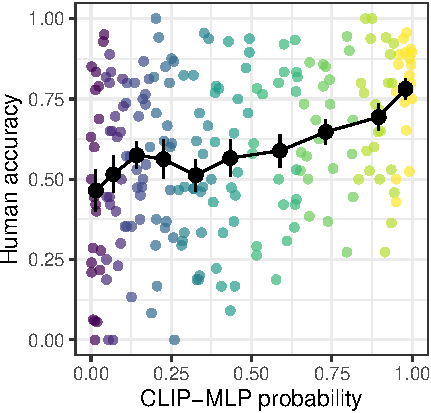
\includegraphics[width=0.7\linewidth]{figs/fig-calibration-1} 

}

\caption[Correlation between human accuracy and CLIP-MLP probability of target in Experiment 1]{Correlation between human accuracy and CLIP-MLP probability of target in Experiment 1.  Points are individual descriptions, colored by decile of CLIP-MLP probability, black line is the bootstrapped mean and 95\% CI across descriptions for each decile. \label{calibration}}\label{fig:fig-calibration}
\end{figure}
\end{CodeChunk}

Our CLIP-MLP computational model was optimized for task accuracy. To
validate whether this objective also results in human-like response
patterns, we conducted a calibration experiment to determine if, for any
given utterance, the model-assigned target probability was aligned with
the probability that a naïve human matcher would choose the target
image.

\subsection{Methods}\label{methods}

We first obtained target probabilities from our CLIP-MLP model for all
utterances from Boyce et al. (2024). We then used stratified sampling to
select 217 trials by dividing model-predicted probabilities into deciles
and choosing approximately 22 utterances per decile, spanning the 12
different possible target images.

We recruited 61 participants who each saw 64 trials randomly sampled
from the 217 tested trials. On average, each trial was seen by 18
participants. This experiment was pre-registered at
\url{https://osf.io/6pv5e}.

\subsection{Results and discussion}\label{results-and-discussion}

We obtained human accuracies on each trial by dividing the number of
participants who selected the target by the total number of participants
who saw the trial (Figure \ref{fig:fig-calibration}). There was a modest
but significant positive correlation between model-predicted
probabilities and human accuracies (\(r\) = 0.33 {[}0.21, 0.45{]}). This
result suggests that model predictions were calibrated to human response
patterns, albeit not perfectly. It is possible to use these calibration
results to tune model predictions to better approximate human responses;
we leave this approach for future work. Nonetheless, the observed
positive correlation suggests that our computational model carries some
signal about human accuracies, validating its use in subsequent
experiments as a computational comparison.

\begin{CodeChunk}
\begin{figure}[t]

{\centering 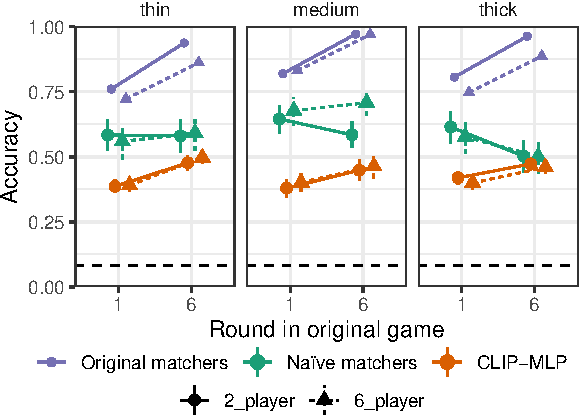
\includegraphics[width=0.9\linewidth]{figs/fig-condition-1} 

}

\caption[Accuracies for naïve human matchers and the CLIP-MLP model for Experiments 2a and 2b, grouped by the source of the referential description]{Accuracies for naïve human matchers and the CLIP-MLP model for Experiments 2a and 2b, grouped by the source of the referential description. Facets are the communication thickness of the original game and x-axis is when in the game the transcript caome form. Point estimates and 95\% CrI are predictions from the fixed effects of logistic and beta regressions. Bootstrapped mean accuracy from the original matchers is included as a ceiling, and random chance as a baseline. \label{expt2-condition}}\label{fig:fig-condition}
\end{figure}
\end{CodeChunk}

\begin{CodeChunk}
\begin{figure}[t]

{\centering 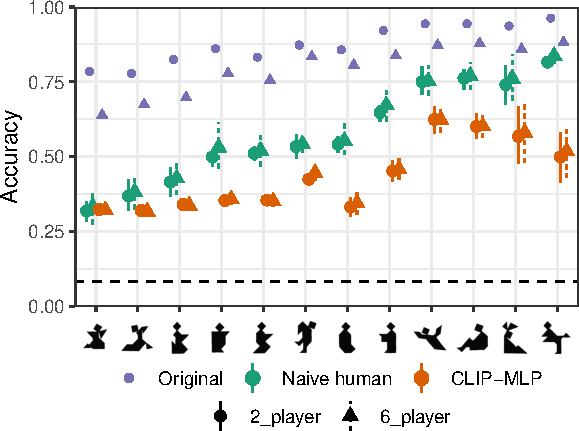
\includegraphics[width=0.9\linewidth]{figs/fig-2-1} 

}

\caption[Accuracies for naïve human matchers and the CLIP-MLP model for Experiments 2a and 2b, split out by target image]{Accuracies for naïve human matchers and the CLIP-MLP model for Experiments 2a and 2b, split out by target image. Point estimates and 95\% CI are predictions from the fixed effects and by-tangram random effects of logistic and beta regressions, bootstrapped across conditions. Bootstrapped mean accuracy from the original matchers is included as a ceiling, and random chance as a baseline. \label{expt2-tangram}}\label{fig:fig-2}
\end{figure}
\end{CodeChunk}

\section{Experiment 2}\label{experiment-2}

As a starting point for examining what makes referential expressions
more or less opaque, we focused on referring expressions from the first
and last rounds of games. Principles of convention formation and
people's behavior when switching to a new partner suggest that
later-round utterances are more opaque and thus harder to understand.
One counterargument is that later rounds are the result of describers'
accumulated practice refining descriptions to be maximally communicative
and to pick out the most visually salient features. To distinguish these
hypotheses, we ran a recognition experiment including descriptions from
games of different sizes and communication thicknesses. Based on the
patterns of cross-game similarity in Boyce et al. (2024), we expected
that smaller and thicker games, whose descriptions diverged fastest,
would have more idiosyncratic and opaque conventions than larger groups
with thinner communication channels.

\subsection{Methods}\label{methods-1}

\subsubsection{Experiment 2a}\label{experiment-2a}

To establish a baseline of how well naïve matchers could understand
descriptions without context, we ran a 2x2 within subjects experiment.
We drew the target transcripts from 2- and 6-player games from
Experiment 1 of Boyce et al. (2024) and from the first and last blocks
of these games. These games had medium-thick communication channels,
where matchers could send text messages to the shared chat interface,
but the describer role rotated each round, and matchers received limited
feedback. We recruited 60 participants who each saw 60 trials (15 in
each of the 4 conditions). Overall, participants saw 774 transcripts
from 40 games. This experiment was pre-registered at
\url{https://osf.io/k45dr}.

\subsubsection{Experiment 2b}\label{experiment-2b}

After observing limited condition differences in Experiment 2a, we ran a
follow-up experiment on descriptions from Experiment 3 of Boyce et al.
(2024), where the communication channel thicknesses were more extreme.
Here, we used a 2x2x2 within subjects design, drawing our transcripts
from the first and last rounds of thick and thin, 2- and 6- person
games. In the ``thick'' condition, matchers could send text messages to
the shared chat interface, one person was the the describer role the
whole game, and matchers recived feedback on everyone's selections. In
contrast, in the ``thin'' condition, original matchers could only
contribute to the chat by sending one of 4 emojis, the describer role
rotated, and matchers recieved limited feedback. As the emojis did not
have referential content, we did not include them in the transcripts
shown to naïve matchers. For experiment 2b, we recruited 60 participants
who each saw 64 trials (8 in each of the 8 conditions). Overall,
participants saw 2392 transcripts from 163 games. This experiment was
pre-registered at \url{https://osf.io/rdp5k}.

\subsection{Results}\label{results}

\subsubsection{Experiment 2a}\label{experiment-2a-1}

For Experiment 2a, we ran a Bayesian mixed effects logistic model of
naïve matcher accuracy in brms (Bürkner, 2018).\footnote{correct
  \({\sim}\) group\_size \({\times}\) round~\({+}\) trial\_order~\({+}\)
  (group\_size \({\times}\) round\textbar correct\_tangram)~\({+}\)
  (group\_size \({\times}\) round~\({+}\) trial\_order\textbar workerid)}
Overall, naïve matchers were right 62\% of the time, which was far above
the 1/12 = 8.3\% expected by random chance (OR = 1.93 {[}1.05, 3.62{]}).
There were not large effects of condition (Figure \ref{expt2-condition}
middle panel). Participants tended to be less accurate at descriptions
from the last round (OR of last round = 0.77 {[}0.53, 1.10{]}). There
was not a clear effect of original group size (OR of 6-player game =
1.15 {[}0.89, 1.47{]}), but there was an interaction between round and
group size (OR = 1.49 {[}1.06, 2.10{]}). Later transcripts from larger
games were easier to understand, but earlier transcripts from smaller
games were easier to understand. Much of the variation in accuracy was
driven not by condition, but by the target image (OR of standard
deviation of image distribution = 2.66 {[}1.88, 4.52{]}). Some images
were much easier to identify as the target than others (Figure
\ref{expt2-tangram}).

\subsubsection{Experiment 2b}\label{experiment-2b-1}

For Experiment 2b we ran a similar Bayesian mixed effects logistic
model.\footnote{correct \({\sim}\) group\_size \({\times}\) thickness
  \({\times}\) round~\({+}\) trial\_order~\({+}\) (group\_size
  \({\times}\) thickness \({\times}\)
  round\textbar correct\_tangram)~\({+}\) (group\_size \({\times}\)
  thickness \({\times}\) round~\({+}\) trial\_order\textbar workerid)}
Naïve matchers were above chance (OR = 1.81 {[}1.06, 3.08{]}, Figure
\ref{expt2-condition} ). Similar to experiment 2a, there were not
substantial effects of condition. Last round descriptions had slightly
lower accuracy (OR of last round = 0.64 {[}0.47, 0.85{]}), but there was
an interaction with thickness, where for thin games, last round
descriptions were less opaque (OR = 1.55 {[}1.02, 2.33{]}). Again some
of the uncertainty in estimating the fixed effects was driven by the
strong variation based on target image (OR of SD of images = 2.25
{[}1.67, 3.59{]}, Figure \ref{expt2-tangram}).

\subsubsection{Additional predictors}\label{additional-predictors}

As additional post-hoc predictors, we examined the accuracy of the
in-game matchers from Boyce et al. (2024) and the length of the
description. In both experiments, in-game accuracy was predictive of
naïve matcher accuracy (Expt 2a OR = 3.33 {[}2.45, 4.53{]}, Expt 2b OR =
2.39 {[}1.88, 3.03{]}). The log number of words in the description was
not predictive in Experiment 2a (OR = 1.05 {[}0.94, 1.17{]}), but longer
descriptions were slightly beneficial in Experiment 2b (OR = 1.10
{[}1.01, 1.20{]}).

\subsection{Model results}\label{model-results}

As a computational comparison, we looked at the CLIP-MLP model's
performance on the same descriptions. We used the probability the model
assigned to the correct target as our dependent measure and fit a
Bayesian mixed effects beta regression on the descriptions from
Experiment 2.\footnote{correct \({\sim}\) group\_size \({\times}\)
  thickness \({\times}\) round~\({+}\) (group\_size \({\times}\)
  thickness \({\times}\) round\textbar correct\_tangram)} The CLIP-MLP
model was far above chance, but had lower accuracy than the human
participants (OR = 0.60 {[}0.45, 0.82{]}).

None of the fixed effects in the model were significant, and there was
wide uncertainty for all of them. There was substantial by-target image
variation (1.58 {[}1.31, 2.15{]}) and substantial by-target variation in
the effect of later round (1.56 {[}1.29, 2.09{]}).

As additional predictors, we checked the effect of in-game matcher
accuracy and the length of the description. CLIP-MLP had higher accuracy
when in-game matcher accuracy was higher (OR = 1.52 {[}1.35, 1.71{]}),
and the model did better on shorter descriptions (OR for log words =
0.85 {[}0.82, 0.90{]}). Long descriptions may be more difficult because
they are further further from the model's training distribution of image
captions.

\subsection{Discussion}\label{discussion}

Overall, naïve human matchers were fairly accurate overall, but less
accurate than matchers in the original game. Perhaps surprisingly, this
level of accuracy was fairly consistent across descriptions from
different times in the game and different game conditions. Accuracy rose
from earlier to later rounds for human matchers in the 6-player medium
condition. The reverse was true for human matchers reading descriptions
from 2-player medium games and both thick conditions, and human matchers
showed minimal difference across time-points for descriptions from the
thin condition. The largest source of variability in accuracy was from
the target images; while there was some variabiliity in accuracy by
images for the original matchers, there was substantially more
variability for naïve matchers. The computational model showed a similar
pattern of large effects of image, but had overall lower accuracy than
naïve human matchers.

\section{Experiment 3}\label{experiment-3}

The experiment of naïve matchers in Experiment 2 differed from in-game
matchers in several ways. In-game matchers recieved descriptions from a
consistent group, recieved descriptions in the order they were created,
and were present participants during the game. In Experiment 3, we focus
on the role of context and group-specific interaction history to tease
apart some of these differences.

\subsection{Methods}\label{methods-2}

We compared naïve matchers in ``yoked'' and ``shuffled'' conditions. In
the ``yoked'' condition, naïve matchers saw all the descriptions from a
single game in the order they originally occurred. In the ``shuffled''
condition, naïve matchers saw all the descriptions from a single game in
a randomized order. This is the same yoking but a different shuffling
than that used in Hawkins et al. (2023).

Because some descriptions are already fairly comprehensible in
isolation, we focused on the role of context for games that showed
strong group-specificity. We hand-picked 10 games from Boyce et al.
(2024) on the basis of high in-game matcher accuracy, strong patterns of
descriptions shortening over repetition, and the use of idiosyncratic or
non-modal referring expressions. Thus, these games showed the hallmarks
of strong conventionalization to terms that were more likely to be
opaque to outsiders.

We recruited 196 participants (99 in the yoked condition and 97 in
shuffled) who each saw all 72 trials of one of the 10 games. This
experiment was pre-registered at \url{https://osf.io/zqwp5}.
Participants read the transcripts in a modified self-paced reading
procedure where they uncovered the text word by word (revealed words
stayed visible); only after uncovering the entire transcript could
participants select an image. We do not analyze the reading time data
here.

\begin{CodeChunk}
\begin{figure}[t]

{\centering 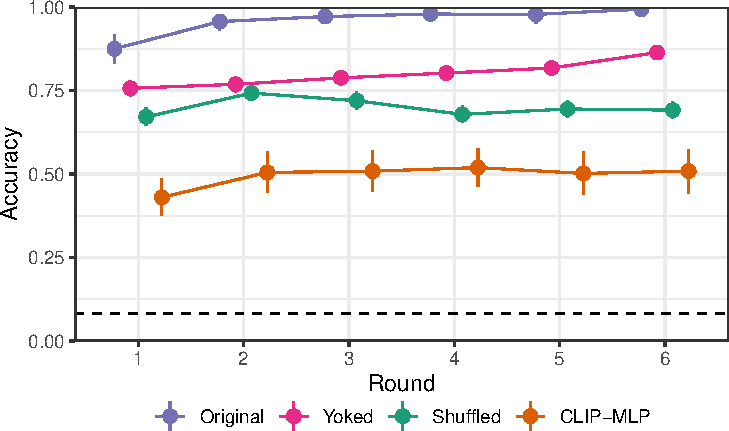
\includegraphics[width=0.9\linewidth]{figs/fig-yoked-1} 

}

\caption[Accuracies for Experiment 3]{Accuracies for Experiment 3. Error bars are bootstrapped 95\% CIs. TODO not using predictions because those fuzz out round to round differences. \label{yoked}}\label{fig:fig-yoked}
\end{figure}
\end{CodeChunk}

\subsection{Results and discussion}\label{results-and-discussion-1}

Our primary question of interest was how much having the conversation
history would help make later round descriptions more understandable to
participants in the yoked condition.

We compared accuracy across the yoked and shuffled conditions with a
Bayesian mixed effects logistic regression.\footnote{correct \({\sim}\)
  orig\_repNum \({\times}\) condition~\({+}\) matcher\_trialNum~\({+}\)
  (1\textbar gameId)~\({+}\) (1\textbar correct\_tangram)~\({+}\)
  (1\textbar workerid)}. The descriptions were more transparent when
they were presented in a yoked order (OR = 2.20 {[}1.63, 3.00{]}, Figure
\ref{yoked}). In the shuffled condition, there was no main effect of
round number (OR for one round later = 0.99 {[}0.95, 1.02{]}), but there
was a marginal interaction where the benefit of the yoked condition
decreased for later rounds (OR for one round later = 0.94 {[}0.89,
1.00{]}). This was offset by matchers in both conditions improving at
the task over time (OR for one trial later in matcher viewing order =
1.02 {[}1.02, 1.02{]}). In the yoked condition round and trial number
were aligned, so an improvement over time could be either from matcher
practice or from descriptions being easier to understand. In the
shuffled condition, matcher practice effects did not correlate with
position in the original game.

Comparing to the performance of in-game matchers, we can separate out
the benefits of seeing the descriptions in order versus being a
participant in the group.\footnote{correct \({\sim}\) orig\_repNum
  \({\times}\) order~\({+}\) orig\_repNum \({\times}\) setting~\({+}\)
  matcher\_trialNum~\({+}\) (1\textbar gameId)~\({+}\)
  (1\textbar correct\_tangram)~\({+}\) (1\textbar workerid)} There is a
benefit to seeing the items in order (OR = 2.24 {[}1.63, 3.04{]}) and a
larger benefit to being a participant during the game (OR = 4.35
{[}2.77, 6.89{]}). The benefit of seeing the items in order wanes in
later blocks (OR = 0.94 {[}0.89, 1.00{]}), but the benefit of being in
the game does not (OR = 1.06 {[}0.95, 1.18{]}). In all cases, there is a
baseline improvement over trials (OR = 1.02 {[}1.02, 1.02{]}).

The accuracy of the CLIP-MLP model is worse than the shuffled human
results, and does not show change across rounds (OR for one round later
= 1.02 {[}0.97, 1.07{]}). The larger difference between naïve human and
CLIP-MLP accuracies in Experiment 3 than Experiment 2 could suggest that
even the shuffled ordering still provides useful context (e.g., the
consistent set of images) that helps matchers understand the
conventions. This history is not available to the CLIP-MLP model which
sees every description as a one-shot task.

\section{General discussion}\label{general-discussion}

Conventions are formed in reference games in a partner-specific way,
where different groups follow different paths through semantic space as
they form conventions. However, the referential descriptions used over
the course of convention formation remain relatively understandable to
outsiders. Across multiple experiments with human matchers, we found
that naïve human matchers were far above chance accuracy at identifying
the targets, with variation explained more by the target image than the
round or game condition the descriptions came from. Even for games
selected for strong conventionalization, naïve matchers had high
accuracy that was aided if they saw the descriptions in order.

We also tested a computational model built on CLIP with a multi-layer
perceptron readout as a way of approximating the context-independent
semantic distance between descriptions and images. The CLIP-MLP model
was far above chance in its assignment of probabilities to target
images, and although its probabilities were lower than human matcher
accuracies, the model mirrored the qualitative pattern of larger effects
from target image than from description source.

Our experimental and computational results were only on a specific set
of iterated reference game transcripts targeting a specific set of 12
images and so numeric results may not generalize to other reference
games with different array sizes and sets of images. There are potential
non-measured differences between in-game matchers and naïve matchers
because naïve matchers did not have to wait for descriptions to appear
and thus had more choice about how closely to read descriptions or how
long to spend looking at images. We also cannot know whether naïve
matchers (or for that matter, in-game matchers) fully ``comprehended''
the language in the descriptions, or were making inferences about the
meaning on a more analytic level.

This work suggests that conventions formed within a small group may
still be fairly comprehensible to those outside the group, who may
produce different descriptions themselves. This finding raises questions
around how well-calibrated describers are to their matcher's level of
knowledge, and whether the process of convention formation is actually
efficient. Even naïve matchers can often understand the shorthand
descriptions, but in reference games, describers choose elaborated
descriptions with new matchers. In a game, norms of cooperation and
conversation may lead describers to start new matchers with elaborated
descriptions designed to give them a high level of confidence in target
selection. Describers are also constrained by their need to come up with
a description in real time. However, the high level of understanding and
the lack of substantial benefit from early round descriptions does raise
empirical questions about how calibrated describers are to the level of
information necessary.

We found large variation in how accurate the computation model and naïve
matchers were on different target images. This effect raises questions
about what makes some images much easier to identify. They might be more
iconic, with a narrower prior over different ways they could be
conceptualized, or they may be further from competitors within this pool
of images. We are limited by the 12 images we used, but future work
sampling across larger sets of images (such as Ji et al., 2022) could
probe image-level factors. Future work could also explore
within-description sources of variation and how the structure and word
choice of utterance correlates with naïve matcher accuracy.
Computational models could be especially beneficial because they could
be run on subsets or ablations of descriptive text.

\section{References}\label{references}

\setlength{\parindent}{-0.1in} 
\setlength{\leftskip}{0.125in}

\noindent

\phantomsection\label{refs}
\begin{CSLReferences}{1}{0}
\bibitem[\citeproctext]{ref-boyce2024}
Boyce, V., Hawkins, R., Goodman, N. D., \& Frank, M. C. (2024).
\emph{Interaction structure constrains the emergence of conventions in
group communication}.

\bibitem[\citeproctext]{ref-burkner2018}
Bürkner, P.-C. (2018). Advanced bayesian multilevel modeling with the r
package brms. \emph{The R Journal}, \emph{10}(1), 395--411.

\bibitem[\citeproctext]{ref-chen2016xgboost}
Chen, T., \& Guestrin, C. (2016). Xgboost: {A} scalable tree boosting
system. \emph{Proceedings of the 22nd Acm Sigkdd International
Conference on Knowledge Discovery and Data Mining}, 785--794.

\bibitem[\citeproctext]{ref-clark1987a}
Clark, H. H., \& Schaefer, E. F. (1987). Concealing one's meaning from
overhearers. \emph{Journal of Memory and Language}, \emph{26}(2),
209--225. \url{https://doi.org/10.1016/0749-596X(87)90124-0}

\bibitem[\citeproctext]{ref-clark1986}
Clark, H. H., \& Wilkes-Gibbs, D. (1986). \emph{Referring as a
collaborative process}.

\bibitem[\citeproctext]{ref-grand2022}
Grand, G., Blank, I. A., Pereira, F., \& Fedorenko, E. (2022). Semantic
projection recovers rich human knowledge of multiple object features
from word embeddings. \emph{Nature Human Behaviour}, \emph{6}(7),
975--987. \url{https://doi.org/10.1038/s41562-022-01316-8}

\bibitem[\citeproctext]{ref-gul2024}
Gul, M. O., \& Artzi, Y. (2024). \emph{{CoGen}: {Learning} from
{Feedback} with {Coupled Comprehension} and {Generation}}
(arXiv:2408.15992). arXiv.
\url{https://doi.org/10.48550/arXiv.2408.15992}

\bibitem[\citeproctext]{ref-hawkins2020b}
Hawkins, R. D., Frank, M. C., \& Goodman, N. D. (2020). Characterizing
the dynamics of learning in repeated reference games.
\emph{arXiv:1912.07199 {[}Cs{]}}. \url{https://arxiv.org/abs/1912.07199}

\bibitem[\citeproctext]{ref-hawkins2021}
Hawkins, R. D., Liu, I., Goldberg, A. E., \& Griffiths, T. G. (2021).
Respect the code: {Speakers} expect novel conventions to generalize
within but not across social group boundaries. \emph{CogSci}.

\bibitem[\citeproctext]{ref-hawkins2023a}
Hawkins, R. D., Sano, M., Goodman, N. D., \& Fan, J. E. (2023). Visual
resemblance and interaction history jointly constrain pictorial meaning.
\emph{Nature Communications}, \emph{14}(1), 2199.
\url{https://doi.org/10.1038/s41467-023-37737-w}

\bibitem[\citeproctext]{ref-ji2022}
Ji, A., Kojima, N., Rush, N., Suhr, A., Vong, W. K., Hawkins, R., \&
Artzi, Y. (2022). Abstract {Visual Reasoning} with {Tangram Shapes}. In
Y. Goldberg, Z. Kozareva, \& Y. Zhang (Eds.), \emph{Proceedings of the
2022 {Conference} on {Empirical Methods} in {Natural Language
Processing}} (pp. 582--601). Association for Computational Linguistics.
\url{https://doi.org/10.18653/v1/2022.emnlp-main.38}

\bibitem[\citeproctext]{ref-kang2020}
Kang, Y., Wang, T., \& de Melo, G. (2020). Incorporating {Pragmatic
Reasoning Communication} into {Emergent Language}. \emph{Advances in
{Neural Information Processing Systems}}, \emph{33}, 10348--10359.

\bibitem[\citeproctext]{ref-le2022}
Le, H., Daryanto, T., Zhafransyah, F., Wijaya, D., Coppock, E., \& Chin,
S. (2022). \emph{Referring {Expressions} with {Rational Speech Act
Framework}: {A Probabilistic Approach}} (arXiv:2205.07795). arXiv.
\url{https://doi.org/10.48550/arXiv.2205.07795}

\bibitem[\citeproctext]{ref-leeuw2023}
Leeuw, J. R. de, Gilbert, R. A., \& Luchterhandt, B. (2023). {jsPsych}:
{Enabling} an {Open-Source Collaborative Ecosystem} of {Behavioral
Experiments}. \emph{Journal of Open Source Software}, \emph{8}(85),
5351. \url{https://doi.org/10.21105/joss.05351}

\bibitem[\citeproctext]{ref-leung2024}
Leung, A., Yurovsky, D., \& Hawkins, R. D. (2024). Parents spontaneously
scaffold the formation of conversational pacts with their children.
\emph{Child Development}, \emph{n/a}(n/a).
\url{https://doi.org/10.1111/cdev.14186}

\bibitem[\citeproctext]{ref-murfitt2001}
Murfitt, T., \& McAllister, J. (2001). The {Effect} of {Production
Variables} in {Monolog} and {Dialog} on {Comprehension} by {Novel
Listeners}. \emph{Language and Speech}, \emph{44}(3), 325--350.
\url{https://doi.org/10.1177/00238309010440030201}

\bibitem[\citeproctext]{ref-muttenthaler2021}
Muttenthaler, L., \& Hebart, M. N. (2021). {THINGSvision}: {A Python
Toolbox} for {Streamlining} the {Extraction} of {Activations From Deep
Neural Networks}. \emph{Frontiers in Neuroinformatics}, \emph{15}.
\url{https://doi.org/10.3389/fninf.2021.679838}

\bibitem[\citeproctext]{ref-ohmer2022}
Ohmer, X., Franke, M., \& König, P. (2022). Mutual {Exclusivity} in
{Pragmatic Agents}. \emph{Cognitive Science}, \emph{46}(1), e13069.
\url{https://doi.org/10.1111/cogs.13069}

\bibitem[\citeproctext]{ref-pedregosa2011scikit}
Pedregosa, F., Varoquaux, G., Gramfort, A., Michel, V., Thirion, B.,
Grisel, O., Blondel, M., Prettenhofer, P., Weiss, R., Dubourg, V., et
al. (2011). Scikit-learn: {Machine} learning in python. \emph{The
Journal of Machine Learning Research}, \emph{12}, 2825--2830.

\bibitem[\citeproctext]{ref-radford2021}
Radford, A., Kim, J. W., Hallacy, C., Ramesh, A., Goh, G., Agarwal, S.,
Sastry, G., Askell, A., Mishkin, P., Clark, J., Krueger, G., \&
Sutskever, I. (2021). \emph{Learning {Transferable Visual Models From
Natural Language Supervision}} (arXiv:2103.00020). arXiv.
\url{https://doi.org/10.48550/arXiv.2103.00020}

\bibitem[\citeproctext]{ref-schober1989}
Schober, M. F., \& Clark, H. H. (1989). Understanding by addressees and
overhearers. \emph{Cognitive Psychology}, \emph{21}(2), 211--232.
\url{https://doi.org/10.1016/0010-0285(89)90008-X}

\bibitem[\citeproctext]{ref-wilkes-gibbs1992}
Wilkes-Gibbs, D., \& Clark, H. (1992). Coordinating beliefs in
conversation. \emph{Journal of Memory and Language}, 183--194.

\bibitem[\citeproctext]{ref-yoon2018}
Yoon, S. O., \& Brown-Schmidt, S. (2018). Aim {Low}: {Mechanisms} of
{Audience Design} in {Multiparty Conversation}. \emph{Discourse
Processes}, \emph{55}(7), 566--592.
\url{https://doi.org/10.1080/0163853X.2017.1286225}

\end{CSLReferences}

\bibliographystyle{apacite}


\end{document}
